% Modle pour rapport de Travail de Fin d'Etudes de l'Ecole Centrale de Lyon
% version 0.1
% 2009-07-24
% par Steren Giannini (steren.giannini@gmail.com)
% Ce modèle est mis  disposition selon le Contrat "Creative Commons
% Paternité-Partage des Conditions Initiales  l'Identique 3.0 Unported"
% http://creativecommons.org/licenses/by/3.0/

\documentclass[12pt,a4paper]{article}
%Chargement des packages
\usepackage[utf8]{inputenc}
\usepackage[french]{babel} %le rapport est en français 
\usepackage{amsmath}
\usepackage{amsfonts}
\usepackage{amssymb}
\usepackage{graphicx} %pour afficher des images
\usepackage{float}    %pour forcer le placement des images.
\usepackage{geometry} %pour la modification des marges
\usepackage{fancyhdr} %pour modification des pieds de page
\usepackage{longtable}
\usepackage{listings}
\usepackage{subfigure}
\usepackage{hyperref} %pour que les références soient des liens hypertextes
\usepackage[usenames,dvipsnames]{color} % pour les textes en gris


% Comment utiliser :
% - la page de titre est à personnaliser (title/title.tex)
% - le contenu est à rédiger dans le répertoire pages/, s'inspirer des exemples
%   présents dans ce modèle.
% - les annexes sont à rédiger dans le répertoire appendix/
% - la bibliographie utilise BibTex (fichier biblio.bib)
% - les variables suivantes sont à remplir :
\newcommand{\TitreRapport}{Rassemblement d'agents mobiles}
\newcommand{\DateRapport}{Mai 2014}
\newcommand{\AuteurRapport}{\'Eloi Perdereau}
\newcommand{\NomEntreprise}{Laboratoire d'informatique fondamentale}

%définition des marges
\geometry{margin=2cm}

%utilisation des puces anglaises.
%attention, il faut avoir une version récente de frenchb.ldf.
\frenchbsetup{StandardItemLabels}

%Définition des en-têtes et pieds de page
\renewcommand{\headrulewidth}{0pt}
\renewcommand{\footrulewidth}{0.5pt}
% \fancyhead[L]{{\small\TitreRapport}}
\fancyfoot[C]{\small\TitreRapport}
\fancyfoot[L]{\small\AuteurRapport}
\fancyfoot[R]{\thepage}

% définition du titre, de la date et de l'auteur du document
\title{\TitreRapport}
\date{\DateRapport}
\author{\AuteurRapport}

\makeatletter

\renewcommand\maketitle{
  \begin{titlepage}
    \begin{center}
      
\includegraphics[width=7.2cm]{title/images/logo_AMU.png}
      \hspace{\stretch{1}}
      
\includegraphics[width=7.2cm]{title/images/logo_LIF.png}

    \vspace{\stretch{0.2}}

      \begin{tabular*}{1.0\textwidth}{l @{\extracolsep{\fill}} r}
          Département Informatique et Interactions & \NomEntreprise \\
          TER \@date                               & Marseille      \\
      \end{tabular*}

    \vspace{\stretch{1.5}}

      {\large \bf Rapport de Travail Encadré de Recherche \\}
      \vspace{0.5cm}
      {\LARGE \bf \@title\\}
      \vspace{0.5cm}
      {\large \it \@author\\}

    \vspace{\stretch{2}}
      
\includegraphics[width=1.0\textwidth]{title/images/logo_illustration.png}
    \vspace{\stretch{2}}

      \begin{tabular}{rl}
        \textit{Tuteur}~:          & Shantanu Das  \\
        \textit{Responsable TER}~: & Omar Boucelma \\
      \end{tabular}

%       \begin{tabular*}{1.0\textwidth}{|l @{\extracolsep{\fill}} r|}
%         \hline
%           Tuteurs :             & Option : (sigle développé)  \\
%           &\\
%           \textit{ECL} :        &                             \\
%           Nom, Prénom Tuteur 1  & Filière : (sigle développé) \\
%           Nom, Prénom Tuteur 2  &                             \\
%           &\\
%           \textit{Entreprise} : &                             \\
%           Nom, Prénom Tuteur 1  & Métier : (sigle développé)    \\
%           Nom, Prénom Tuteur 2  &                             \\
%         \hline
%       \end{tabular*}

    \end{center}\par

  \end{titlepage}
  \setcounter{footnote}{0}
}

\makeatother


\begin{document}
\pagestyle{fancy}

\maketitle
    \newpage
\section*{Remerciements}

Je tiens à remercier mon tuteur, Mr Shantanu Das qui m'a été d'une aide
précieuse tout au long du projet, en m'accordant son temps et en m'apportant
ses connaissances et son expérience du monde de la recherche.

    \newpage
\section*{Résumé du rapport :}
Insérez ici le résumé en français

\subsubsection*{Mots-clés libres :}
Insérez ici les mots clés en français (séparés par des points-virgules)

    \newpage
\section*{Abstract:}
Insérez ici le résumé en anglais

\subsubsection*{Keywords:}
Insérez ici les mots clés en anglais (séparés par des points-virgules)

    \newpage
\tableofcontents
        \newpage
\listoffigures
\listoftables
    \newpage
\section*{Introduction}
\addcontentsline{toc}{section}{Introduction}
Dans le cadre de ma première année de Master informatique à Aix-Marseille
Univsersité (site de Luminy), je suis amené à faire un projet (TER) encadré par
un chercheur d'AMU ou un stage en entreprise. Ayant plus une vocation liée à la
recherche, je me suis orienté vers un projet mêlant programmation et théorie
fondamentale. \\

Le projet rentre dans le domaine de l'algorithmique distribuée~; branche de
l'informatique théorique dont le but est de développer des algorithmes pour des
systèmes distribués impliquant plusieurs processus interconnectés par un
réseau. Ces processus indépendants interagissent et coopèrent entre eux en vue
de réaliser une tâche donnée.  L'idée principal du calcul distribué est que les
processus communiquent entre eux par l'envoi de messages. Néanmoins, nous nous
intéressons ici à un paradigme légèrement différent : les \textit{agents
mobiles}. Ce sont des programmes qui peuvent se déplacer de n\oe{}uds en
n\oe{}uds à l'intérieur du réseau de manière autonome. Bien qu'ils peuvent être
implémentés via le modèle précédent (et font donc parti du calcul distribué),
ils fournissent une abstraction plutôt naturelle pour le développement
d'algorithmes tels que la détection d'intrus, l'exploration d'un réseau
inconnu, ou encore la formation d'un motif par des robots (\textit{robot
pattern formation problem}). Ce dernier problème consiste à arranger les robots
dans le plan pour qu'ils forment et conservent un motif donné. \\

L'objectif ici est de développer et d'implémenter une solution pour un cas
particulier de ce problème~: le rassemblement d'agents mobiles. Aussi appelé le
\GatheringProblem, beaucoup de contributions y ont déjà été apporté, impliquant
souvent un plan continu ou une visibilité infinie. Nous nous restreignons ici à
un espace discret et une visibilité constante des robots. De plus, le système
est synchrone, c'est à dire qu'il existe une horloge globale partagée par tous
les processus. Autrement dit, les algorithmes fonctionneront par
\textit{rondes} (ou \textit{étapes}.) Pour notre cas, cela signifie que tous
les robots décident et se déplacent en même temps.

Le travail à réaliser dans ce projet est donc la recherche des cas de voisinage
et de déplacement des robots pour le \GatheringProblem dans notre contexte. Il
faut également développer une application permettant la visualisation des
robots et de l'algorithme distribué. Cette partie sera faite en utilisant le
langage Python et la librairie TKinter pour l'interface graphique. \\

Dans un premier temps je vais vous présenter plus en détail le sujet et les
outils utilisés~; puis je vous exposerais le travail que j'ai réalisé
développant les différentes étapes de recherche d'un algorithme correct ainsi
que les techniques d'implémentation utilisés. Enfin, je conclurai par un bilan
personnel et professionnel.

        \newpage
\section{Titre1}

Non ergo erunt homines deliciis diffluentes audiendi, si quando de amicitia, quam nec usu nec ratione habent cognitam, disputabunt \footnote{Exemple de note de bas de page}.

\subsection{Titre de niveau 2}

Isdem diebus Apollinaris Domitiani gener, paulo ante agens palatii Caesaris curam, ad Mesopotamiam missus a socero per [...].

\subsubsection{Titre de niveau 3}
Isdem diebus Apollinaris Domitiani gener, paulo ante agens palatii Caesaris curam, ad Mesopotamiam missus a socero per militares numeros immodice scrutabatur, an quaedam altiora meditantis iam Galli secreta susceperint scripta, qui conpertis Antiochiae gestis per minorem Armeniam lapsus Constantinopolim petit exindeque per protectores retractus artissime tenebatur.

\begin{itemize}
\item Liste a puces 1
			\begin{itemize}
			\item Liste a puces 2
						\begin{itemize}
						\item Liste a puces 3
						\end{itemize}
			\end{itemize}
\end{itemize} 

\paragraph{Titre de niveau 4}
Non ergo erunt homines deliciis diffluentes audiendi, si quando de amicitia, quam nec usu nec ratione habent cognitam, disputabunt.

\begin{figure}[H]
	\center
	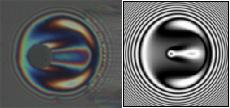
\includegraphics[width=5cm]{body/images/figure_example.png} 
	\caption{Exemple de figure avec légende}
	\label{fig:exemple}
\end{figure}

\subparagraph{Titre de niveau 5}

Isdem diebus Apollinaris Domitiani gener, paulo ante agens palatii Caesaris curam, ad Mesopotamiam missus a socero per militares numeros immodice scrutabatur, an quaedam altiora meditantis iam Galli secreta susceperint scripta, qui conpertis Antiochiae gestis per minorem Armeniam lapsus Constantinopolim petit exindeque per protectores retractus artissime tenebatur.

Titre de niveau 6
Non ergo erunt homines deliciis diffluentes audiendi,


\subsection{Titre de niveau 2}

Isdem diebus Apollinaris Domitiani gener, paulo ante agens palatii Caesaris curam, ad Mesopotamiam missus a socero per [...].


        \newpage
\section{Titre2}

Non ergo erunt homines deliciis diffluentes audiendi, si quando de amicitia, quam nec usu nec ratione habent cognitam, disputabunt.

Exemple de citation \cite{sheffer2006mpm}

    \newpage
\section*{Conclusion}
\addcontentsline{toc}{section}{Conclusion}
Insérez ici votre conclusion.

    \newpage
\bibliographystyle{unsrt}
\bibliography{biblio}
    \newpage
\appendix
\section{Cas de mouvement}

Sans les cas symétriques (rotation)


\end{document}
